\iffalse
\chapter{2014}
\author{AI24BTECH11014}
\section{ce}
\fi

%\begin{enumerate}
    \item An isolated three-phase traffic signal is designed by Webster's method. The critical flow ratio for three phases are $0.20, 0.30,$ and $0.25$ respectively, and lost time per phase is 4 seconds. The optimum cycle length (in seconds) is \underline{\hspace{1cm}}.
 
\item A levelling is carried out to establish the Reduced Levels (RL) of point R with respect to the Bench Mark (BM) at P. The staff readings taken are given below. \\
  \begin{table}[h]
        \centering
        \begin{tabular}{|c|c|c|c|c|}
        \hline
        Staff Station & BS & IS & FS & RL \\
        \hline
        P & 1.655m &  &  & 100.000m \\
        \hline
        Q & -0.950m &  & -1.500m & \\
        \hline
        R &  &  & 0.750m & ? \\
        \hline
        \end{tabular}
    \end{table}

If RL of P is +100.000m, then RL (in m) of R is:
    \begin{enumerate}
        \begin{multicols}{2}
            \item $103.355$
            \item $103.155$
            \item $101.455$
            \item $100.355$
        \end{multicols}
    \end{enumerate}

    \item Group I lists tools/instruments, while Group II lists the corresponding surveying methods. Match the tool/instrument with the corresponding method of surveying.
   \begin{table}[h]
        \centering
        \begin{tabular}{ c@{\hskip 1cm }c }
            Group I & Group II \\
            P. Alidade & 1. Chain surveying \\
            Q. Arrow & 2. Levelling \\
            R. Bubble tube & 3. Plain table surveying \\
            S. Stadia hair & 4. Theodolite surveying \\
        \end{tabular}
    \end{table}

    \begin{enumerate}
        \begin{multicols}{2}
            \item P-3; Q-2; R-1; S-4
            \item P-2; Q-4; R-3; S-1
            \item P-1; Q-2; R-4; S-3
            \item P-3; Q-1; R-2; S-4
        \end{multicols}
    \end{enumerate}

    \item A fair (unbiased) coin was tossed four times in succession and resulted in the following outcomes: (i) Head, (ii) Head, (iii) Head, (iv) Head. The probability of obtaining a 'Tail' when the coin is tossed again is:
    \begin{enumerate}
        \begin{multicols}{4}
            \item $0$
            \item $\frac{1}{2}$
            \item $\frac{4}{5}$
            \item $\frac{1}{5}$
        \end{multicols}
    \end{enumerate}


\item The determinant of the matrix $\begin{pmatrix}
0 && 1 && 2 && 3 \\ 1 && 0 && 3 && 0 \\ 2 && 3 && 0 && 1 \\ 3 && 0 && 1 && 2 \end{pmatrix}$ is \underline{\hspace{1cm}}

\item $ z = \frac{2 - 3 i}{-5 + i}$ can be expressed as
\begin{enumerate}
\begin{multicols}{2}
\item $ -0.5 - 0.5i $
\item $-0.5 + 0.5i$
\item $0.5 - 0.5i$
\item $0.5 + 0.5i$
\end{multicols}
\end{enumerate}

\item The integrating factor for the differential equation $\frac{dP}{dt} + k_{2}P = k_{1}L_{0} e^{-k_{1}t}$ is 
\begin{enumerate}
\begin{multicols}{4}
\item $e^{-k_{1}t}$
\item $e^{-k_{2}t}$
\item $e^{k_{1}t}$
\item $e^{k_{2}t}$
\end{multicols}
\end{enumerate}

\item If $\brak{x}$ is a continuous, real valued random variable defined over the interval $\brak{-\infty, + \infty}$ and its occurence is defined by the density function given as: $f\brak{x} = \frac{1}{\sqrt{2 \pi}}b e^{\frac{-1}{2} {\brak{\frac{x - a}{b}}}^{2}}$ where $'a'$ and $'b'$ are the statistical attributes of the random variable $\brak{x}$. The value of the integral $\int_{-\infty}^{a} \frac{1}{\sqrt{2 \pi}}b e^{\frac{-1}{2} {\brak{\frac{x - a}{b}}}^{2}} dx$ is 

\begin{enumerate}
\begin{multicols}{4}
\item $1$
\item $0.5$
\item $\pi$
\item $\frac{\pi}{2}$
\end{multicols}
\end{enumerate}

\item Group I contains representative stress-strain curves as shown in the figure, while Group II gives the list of materials. Match the stress-strain  curves with the corresponding materials.
\begin{center}
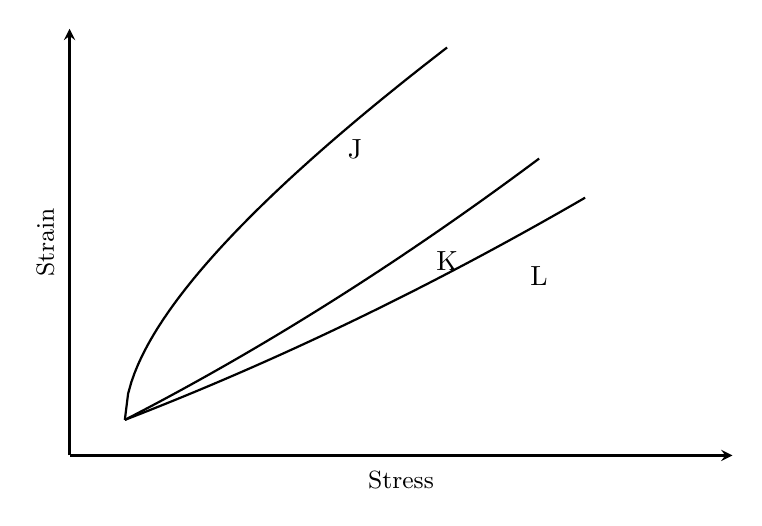
\begin{tikzpicture}
    \begin{axis}[
         xmin=0, xmax=1.2,
        ymin=0, ymax=1.2,
        xtick=\empty, % Remove x-axis tick labels
        ytick=\empty, % Remove y-axis tick labels
        axis x line=bottom,
        axis y line=left,
        enlargelimits=true,
        width=10cm,
        height=7cm,
        xlabel={Stress},
        ylabel={Strain}, 
        label style={font=\small}, 
        axis line style={thick},   ]
        % Curve J
        \addplot[
            thick,
            domain=0:0.7,
            samples=100
        ]
        {x^0.5 + 0.6 * x};
        \node[above] at (axis cs:0.5,0.85) {J}; % Label for Curve J

        % Curve K
        \addplot[
            thick,
            domain=0:0.9,
            samples=100
        ]
        {0.8 * x + 0.2 * x^2};
        \node[below] at (axis cs:0.7,0.6) {K}; % Label for Curve K

        % Curve L
        \addplot[
            thick,
            domain=0:1.0,
            samples=100
        ]
        {0.6 * x + 0.15 * x^2};
        \node[below] at (axis cs:0.9,0.55) {L}; % Label for Curve L
    \end{axis}
\end{tikzpicture}
\end{center}

\begin{table}[h]
\centering
\begin{tabular}{c @{\hskip 1 cm} c}
Group I & Group II \\
P.Curve J & 1.cement paste \\
Q. Curve K & Coarse aggregate \\ 
R. Curve L & 3. Concrete \\

\end{tabular}
\end{table}


    \begin{enumerate}
        \begin{multicols}{2}
            \item P-1; Q-3; R-2; 
            \item P-2; Q-3; R-1; 
            \item P-3; Q-1; R-2; 
            \item P-3; Q-2; R-1; 
        \end{multicols}
    \end{enumerate}

\item The first moment of area about the axis of bending for a beam cross-section is
   \begin{enumerate}
        \begin{multicols}{2}
        \item moment of inertia
        \item section modulus
        \item shape factor
        \item polar moment of inertia 
        \end{multicols}
    \end{enumerate}

\item Polar moment of inertia $\brak{I_{P}}$ , in $cm^{4}$, of a rectangular section having width, $ b = 2 cm $ and depth $ d = 6 cm $  is \underline{\hspace{2cm}} 
\item The target mean strength $f_{cm}$ for concrete mix design obtained from the charecteristic strength $f_{ck}$  and standard deviation $\sigma$, as defined in IS:456-2000, is
    \begin{enumerate}
        \begin{multicols}{2}
            \item $f_{ck} + 1.35 \sigma $
            \item $f_{ck} + 1.45 \sigma $
            \item $f_{ck} + 1.55 \sigma $
            \item $f_{ck} + 1.65 \sigma $
        \end{multicols}
    \end{enumerate}

\item The flexural tensile strength of M25 grade of concrete, in $N/mm^{2}$ as per IS:456-2000 is \underline{\hspace {1 cm}}


%\end{enumerate}

